\chapter{Further statistics details}


\section{Asymptotics approximation}

To emphasize some of the fundamentals of the particle physics statistics that we use, in this section I show my own reproduction of one of the experiments in the asymptotic approximation paper \hl{need to cite}.

Consider a cut-and-count analysis where the signal region (SR) has $s$ signal events, and the background yield is specified by a nuisance parameter (NP) b expected background with $b$ events. Let the number of events that we observe in the SR be $n$, so then the expected value for the observed event yield is: $\mathbb{E}[n] = \mu s +b$. We additionally consider that we have a measurement in a control region where m events are observed, and this control region where the background yield is scaled by $\tau$ relative to the SR, i.e, $\mathbb{E}[m] = \tau b$.

Since this is now just a single bin counting experiment, the likelihood from Eq~{\ref{eq:likelihood}} simplifies to the form:

\begin{equation}
	\mathcal{L}(\mu,b) = \frac{(\mu s + b)^n}{n!} e^{-\mu s+ b} \frac{(\mu s + b)^n}{n!} e^{-\mu s+ b} 
\end{equation}

In this simple example, we can compare the analytic asymptotic formula for the test statistic's distribution to the result from throwing toys to build our intuition for the problem.


\begin{figure}[bht]
	\centering
	\subfloat{
		\label{fig:asymp-3a}
		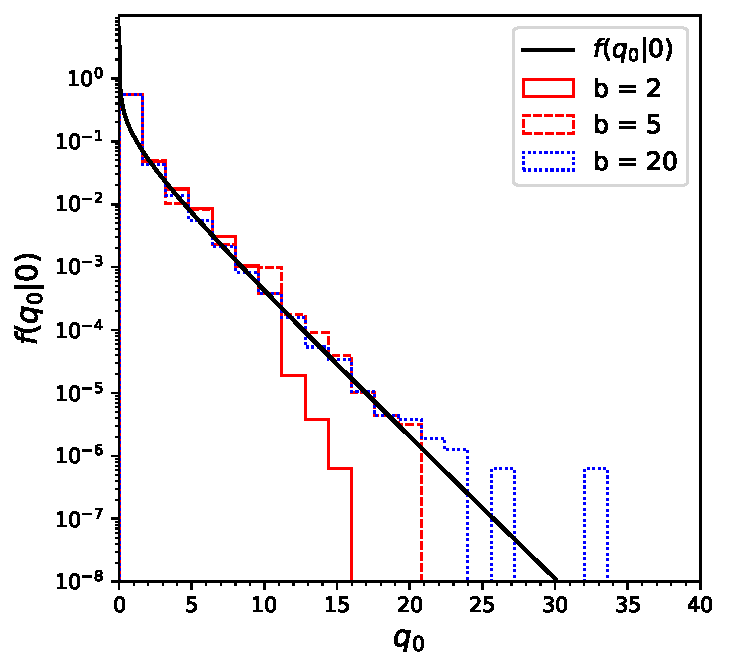
\includegraphics[width=.48\textwidth]{{figures/stats/fig3a.pdf}}
	}
	\subfloat{
		\label{fig:asymp-3b}
		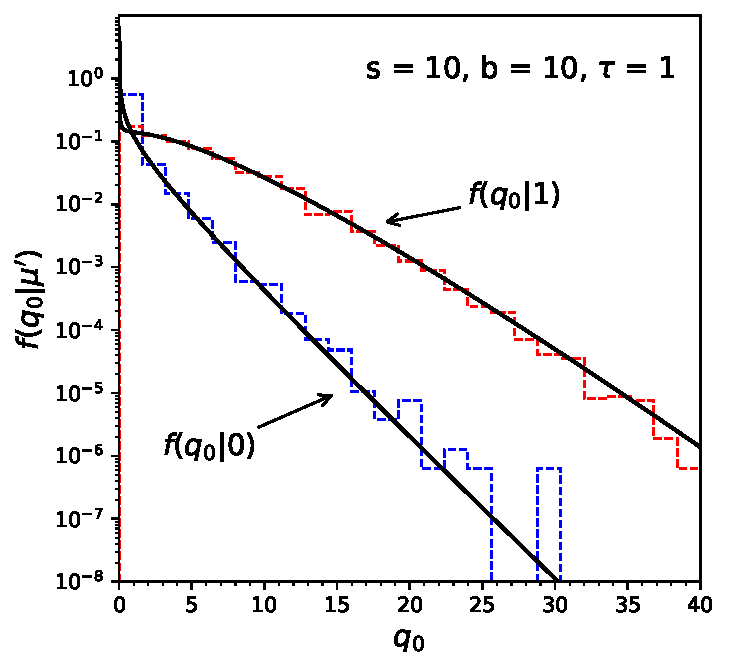
\includegraphics[width=.48\textwidth]{{figures/stats/fig3b.pdf}}
	}
	\caption{}
\end{figure}

\begin{figure}[bht]
	\centering
	\subfloat{
		\label{fig:asymp-4a}
		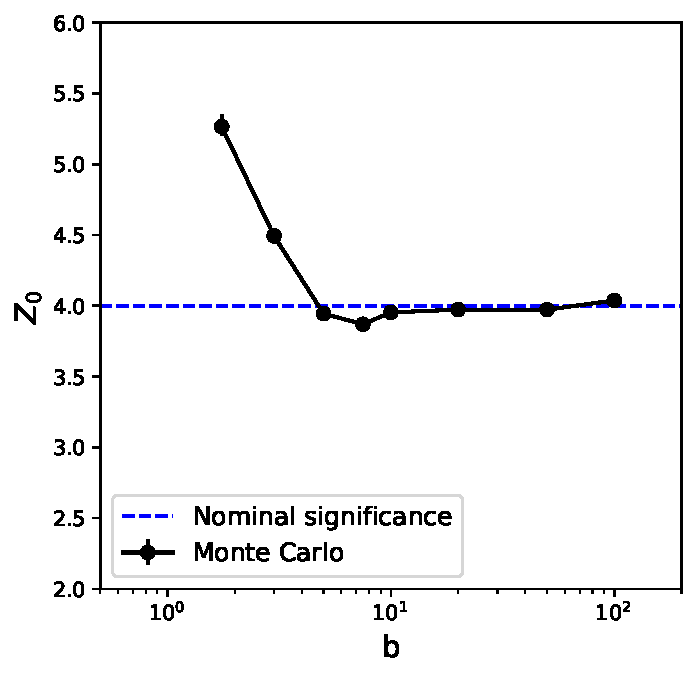
\includegraphics[width=.48\textwidth]{{figures/stats/fig4a.pdf}}
	}
	\subfloat{
		\label{fig:asymp-4b}
		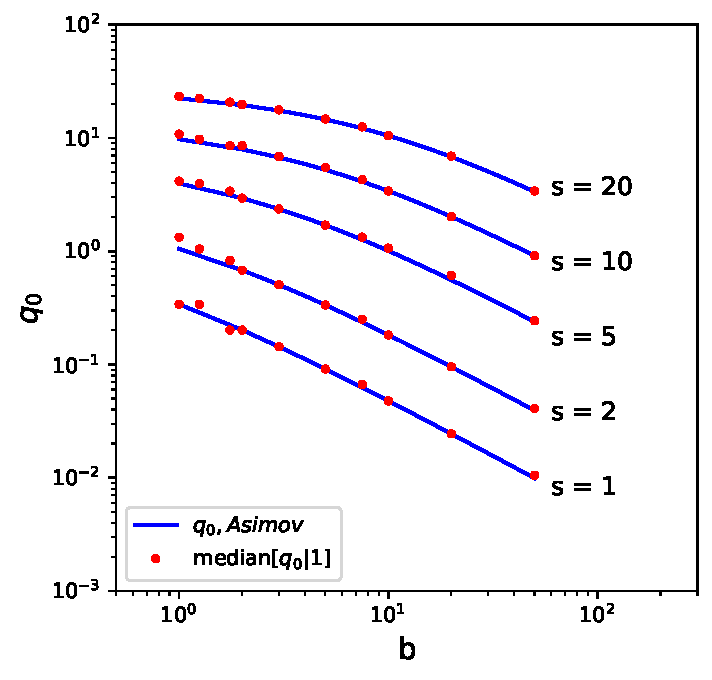
\includegraphics[width=.48\textwidth]{{figures/stats/fig4b.pdf}}
	}
	\caption{}
\end{figure}

\begin{figure}[bht]
	\centering
	\subfloat{
		\label{fig:asymp-5a}
		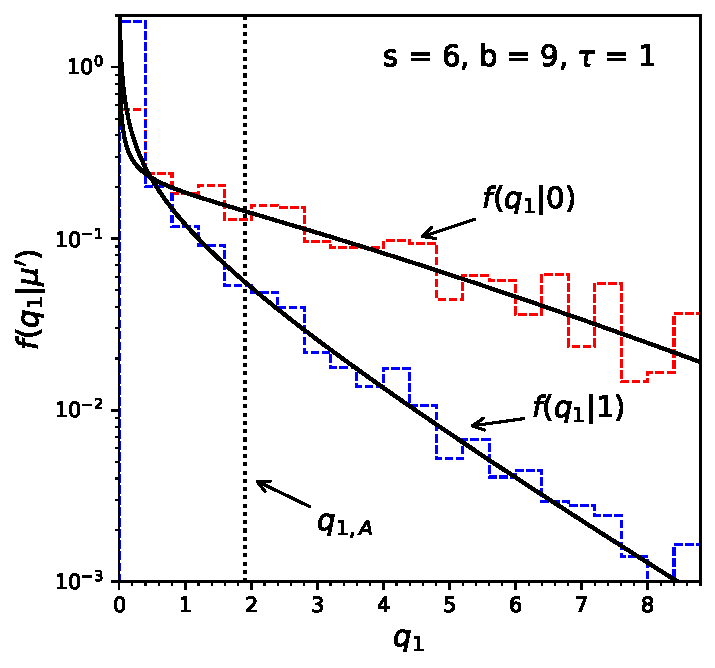
\includegraphics[width=.48\textwidth]{{figures/stats/fig5a.pdf}}
	}
	\subfloat{
		\label{fig:asymp-5b}
		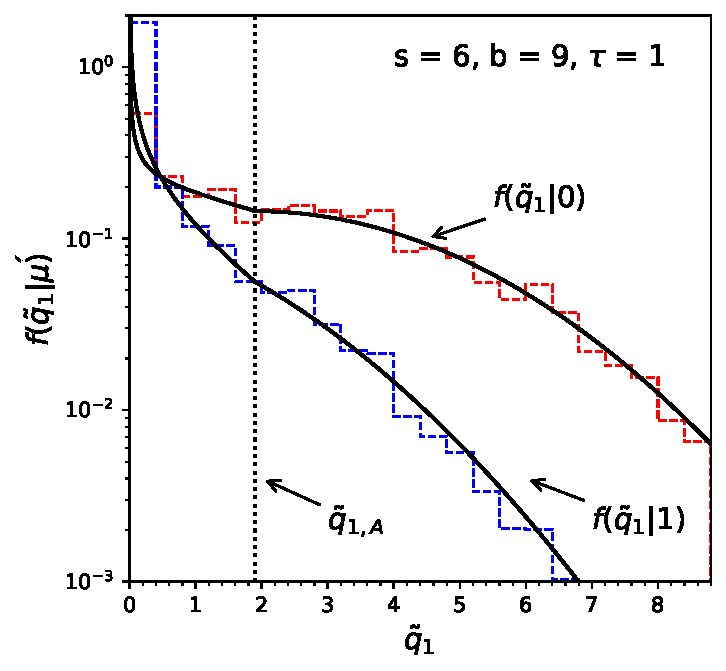
\includegraphics[width=.48\textwidth]{{figures/stats/fig5b.pdf}}
	}
	\caption{}
\end{figure}

\begin{figure}[bht]
	\centering
	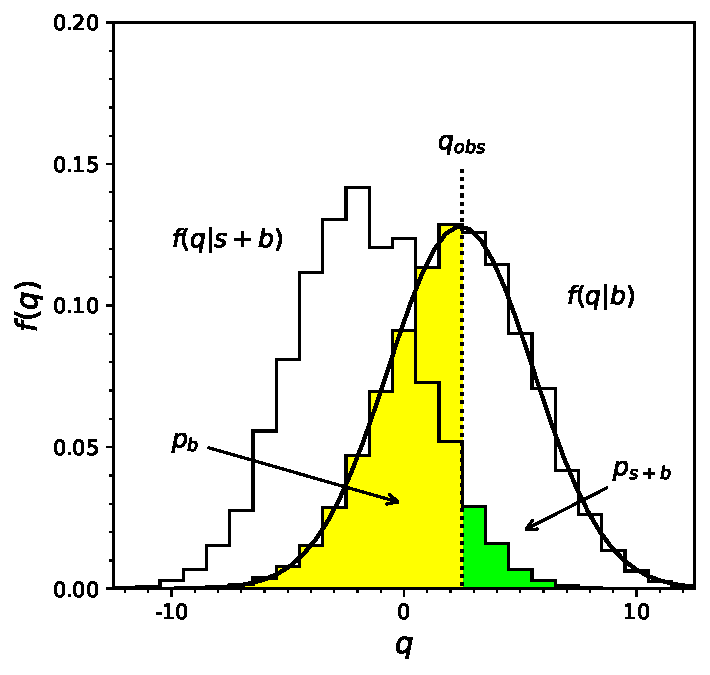
\includegraphics[width=.5\textwidth]{{figures/stats/fig6.pdf}}
	\caption{}
	\label{fig:asymp-6}
\end{figure}

\begin{figure}[bht]
	\centering
	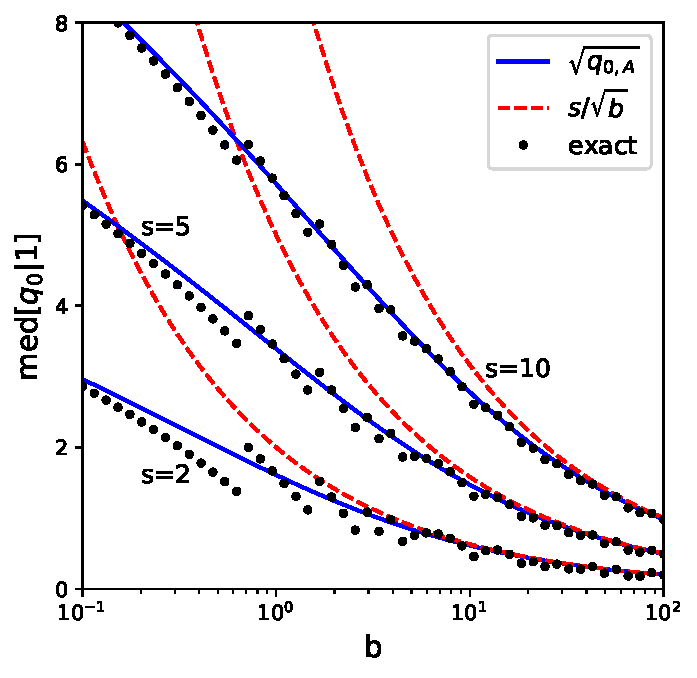
\includegraphics[width=.5\textwidth]{{figures/stats/fig7.pdf}}
	\caption{}
	\label{fig:asymp-7}
\end{figure}

\FloatBarrier
\clearpage

\section{Choice of CLs test statistic}

\subsection{A pedagogical example}

%\hl{need to cite the Statistics III lecture from the ESHEP summer school}

There can be a problem for the frequentist interpretation if the number of observed events is less than the number of predicted events (in our notation, $n_i < b_i$).
As an example of this, consider a Poisson experiment where we expect $b = 8$ background events, but only observe $n = 3$ events (from \cite{eshep-statsIII}. Considering the model where $\mathbb{n} = s+b$, we can calculate the 95\% upper limit on the true expected number of events by summing up the poisson probabilities of observing this many events or fewer (which is what is also defined as $CL_{s+b})$: 
 
\begin{equation}
Prob(\text{observing} \leq 3 \text{events})  = CL_{s+b} = \sum_{r=0}^{3} \frac{ n^r e^{-n}}{r!}.
\end{equation}

\Fig{\ref{fig:CLs-graphic}} (blue line) shows the result of $CL_{s+b}$ as we scan over $n$ values.
By settig $CL_{s+b} = 0.05$, we find $n = 7.75$. % $ \sum_{r=0}^{3} \frac{7.75^r e^{-7.75}}{r!} = 0.05$
Then solving for an upper limit on the signal yield, we get $s$, we get $s = n - b = n - 8 = - 0.25$, an unphysical result.

\begin{figure}[bht]
	\centering
	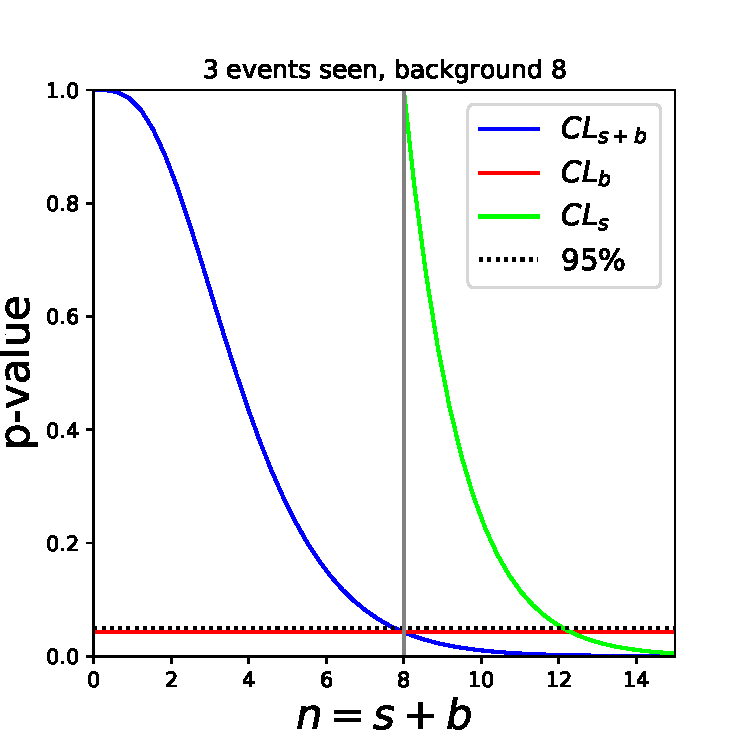
\includegraphics[width=.5\textwidth]{{figures/stats/Pois_nb_8_nd_3.pdf}}
	\caption{A comparison of the \ldots}
	\label{fig:CLs-graphic}
\end{figure}
 
To avoid the pathologies of the 
 has been a convention that's been used since the Tevatron \hl{need citation}, and is the convention adopted across the HH physics analyses to use this as how we interpret a 95\% upper limit - it corresponds to $CL_s = 0.05$.

You can think of this although this is does mean that we now have a conservative upper limit because
 

\begin{itemize}
\item $CL_{s+b}$: Probability that we saw this number of events (or fewer) given an expected yield of s+b.
\item $CL_b$: Same as $CL_s$,but with $b=0$.
\end{itemize}


\begin{equation}
CL_s = \frac{ CL_{s+b}}{CL_b}
\end{equation}


\subsection{Intuition building - impact on the 4b analysis}



Finally, to illustrate why this was a more conservative choice, 

%%%%%%%%%%%%%%%%%%%%%
% This is the mdr + min dhh pairing alg
%%%%%%%%%%%%%%%%%%%%%
\begin{figure}[bht]
\centering
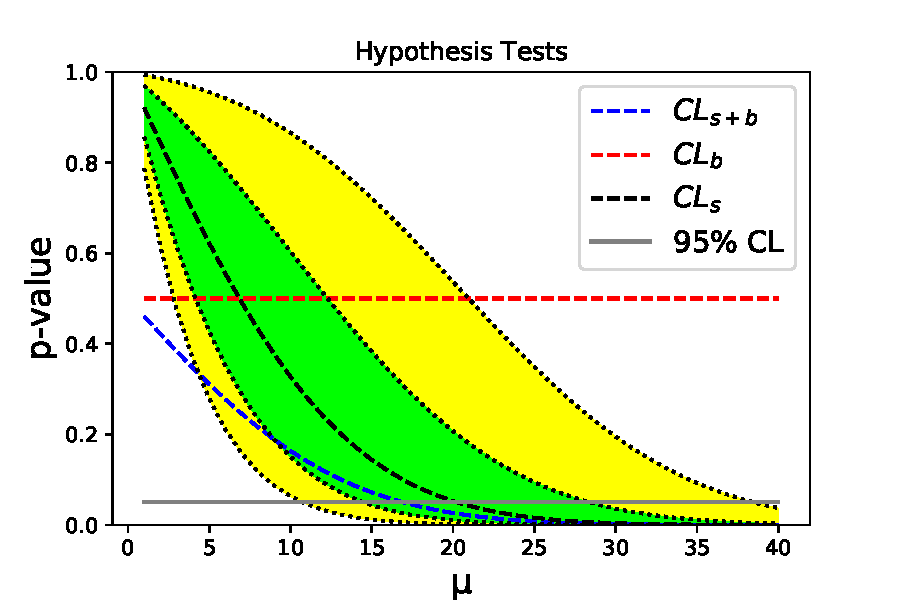
\includegraphics[width=.5 \textwidth]{{figures/stats/cf_scan_mu_CLs+b.pdf}}
\caption{Impact of using the $CL_{s}$ verses the $CL_{s+b}$ test statistic.}
\label{fig:cf-scan-cls+b-HH4b}
\end{figure}